% !TEX root = draft.tex
\chapter{强化学习 ，“强”在哪里？}
(Reinforcement Learning)：通过与环境互动学习策略


 强化学习的背景
 
前面我们感性认知了机器学习的三大门派（监督学习、非监督学习、半监督学习）。在传统的机器学习分类中，并没有包含强化学习。但实际上，在连接主义学习中，还有一类人类学习常用、机器学习也常用的算法—强化学习（ReinforcementLearning，简称RL）。

机器学习的本质，在于改善机器的“智能”水平。那我们就要问问，什么是智能了。关于智能的定义很多，正所谓“仁者见仁，智者见智”。比如说，中国另一位先哲孟子则说:

“是非之心，智也”《孟子·告子上》。
孟子认为，能分辨是非得失，就是有智能的表现。

而这里的“是非”之别，在西方，可用莎士比亚的名句 “to be or not to be”来浓缩，两者之间的活动——“应该”（should）即是智能。

在智能里，它既包含了逻辑，同时也包含了大量的非逻辑成分，比如说模糊、直觉、非公理等因素。

哈弗大学罗兰科学研究所（Rowland Institute for Science）教授威尔逊 (Stewart Willson)对此也有自己独到的见解。他认为[1]，关于对智能的认识，我们应当向大自然学习。

在大自然中，智能的表现，与生物体对生存的需求紧密相关。正是生存的压力和动力，不断划清自然界中的不同问题，并逐步习得解决这些问题的能力，从而使得生物表现出多样性，进而也表现出不同层面的智能。

其实，威尔逊教授的核心观点说的是，从环境中交互获得智能。而“强化学习”就是一种从环境交互中改善自己性能的机器学习方式。


强化学习是一种通过与环境互动来学习最优决策策略的机器学习范式。与监督学习和无监督学习不同，强化学习不依赖于标注数据，而是通过智能体与环境的互动来获取反馈信号，从而学习最优决策策略。智能体需要在状态空间~$S$ 选择动作~$A$，并根据环境给予的奖励信号~$R$（如分数、收益） 调整决策策略，最终的目标是最大化累积奖励~$R$。

在强化学习中，智能体的目标是通过试错来最大化累积奖励。学习过程通常通过以下要素进行描述：
\begin{itemize}
\item {\bf 状态（State）:} 表示智能体在某一时刻所处的环境状态，它反映了智能体当前的环境信息。
\item {\bf  动作（Action）:}是智能体在给定状态下选择的行为，决定了智能体与环境的互动方式。
\item {\bf 奖励（Reward）:}是智能体执行某一动作后，环境给予的反馈信号，用于评估该动作的好坏，从而帮助智能体改进其行为。
\item {\bf  策略（Policy）:} 是智能体在特定状态下采取某一动作的规则或函数，智能体通过优化策略来实现目标。
\end{itemize}

强化学习的学习过程通常通过试探和互动来进行，智能体通过不断地探索和利用环境反馈来调整自己的决策策略。这种学习方式非常适用于那些需要长期决策和不断调整行为的复杂任务，如游戏、控制系统和自动驾驶等。与传统的监督学习不同，强化学习无需预定义输入输出对，而是通过与环境的互动动态生成学习信号，学习目标也由环境的反馈动态决定。这种特点使得强化学习能够解决更为复杂和动态的任务。



3.5 什么是强化学习？


强化学习也是机器学习里面非常重要的一个流派。“强化学习”亦称“增强学习”，但它与监督学习和非监督学习都有所不同。强化学习强调的是，在一系列的情景之下，选择最佳决策，它讲究通过多步恰当的决策，来逼近一个最优的目标，因此，它是一种序列多步决策的问题。

强化学习的设计灵感，源于心理学中的行为主义理论：

有机体如何在环境给予的奖励或惩罚刺激下，逐步形成对刺激的预期，从而产生能获得最大利益的习惯性行为。
上面的论述看起来比较抽象，下面我们举一个生活中的例子来说明这个概念。对于儿童教育，有句话非常流行：

“好孩子是表扬出来的”。
这句话是有道理的，它反映了生物体以奖励为动机的行为。比如，我们知道，想让一个小孩子静下来学习，这是十分困难的。但如果父母在他（她）每复习完一篇课文，就说句“你真棒”并奖励一块巧克力，那么孩子就会明白，只有不断学习，才能获得奖励，从而也就更有劲头复习。

“表扬”本身并不等同于监督学习的“教师信号”（即告诉你行为的正误），却也能逐步引导任务向最优解决方案进发。因此，强化学习也被认为是人类学习的主要模式之一。监督学习、强化学习与非监督学习的区别，如图~\ref{监督学习、强化学习与非监督学习的区别}所示。


\begin{figure}[htbp]
\centering
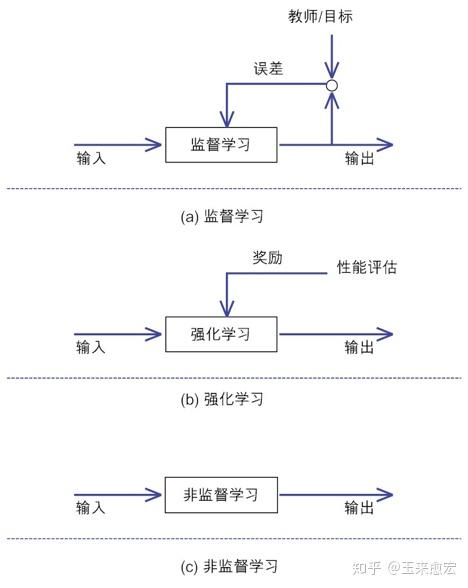
\includegraphics[width=1\textwidth]{figs/监督学习、强化学习与非监督学习的区别.jpg}
\caption{监督学习、强化学习与非监督学习的区别}
\label{监督学习、强化学习与非监督学习的区别}
\end{figure}


3.6 一个形象的例子
恰如其分地拿捏尺度，显然是智能的外在表现之一。“过犹不及”说得就是这个理。那么，强化学习是如何让智能体（Agent）从环境中学习，找到这个“尺度”的呢。下面我们举例[2]来感性认知一下，人类是怎么从环境中学习的。

假设，我们还是一个懵懂的孩子，对于一些新事物一无所知。有一天，我们第一次看到了火，然后就爬到了火堆的旁边。在靠近火的过程中，你感受到了火的温暖，好舒服啊，这时环境给你的回报（reward）为“+1”分。于是，你接着爬向火，越靠越近，然后伸手尝试摸火，好烫啊，环境给你的回报为“-10”分，这是要警告你，你需要赶紧把手缩回来，滚远一点，否则小手就变成“烤猪蹄”了。

这样一来二去，你从“环境”中习得一项智能：距离稍远，火是好东西。靠得太近，火就不是好东西！

这就是人类的学习方式，与环境交互，增强智能。其实，强化学习在理念上和这个是一致的，不同的是，主角变成了计算机（智能体）。



3.7 经典的“西瓜”
在外号雅称为“西瓜书”的《机器学习》一书中\cite{周志华2016}，南京大学的周志华教授就用种西瓜的例子来说明“强化学习”的含义，也别有意义。

考虑一下种西瓜的场景。西瓜从播种到瓜熟蒂落，中间要经过很多步骤。首先得选种，然后播种、定期浇水、施肥、除草、杀虫等，最后收获西瓜。这个过程要经过好几个月。如果把收获高品质的西瓜作为辛勤劳作奖赏的话，那么在种瓜过程中实施某个操作（如浇水、施肥等）时，我们并不能立即得到相应的回报，甚至也难以判断当前操作对最终回报（收获西瓜）有什么影响，因为浇水或施肥并不是越多越好。

然而，即使我们一下子还不能看到辛勤劳作的最终成果，但还是能得到某些操作的部分反馈。例如，瓜秧是否更加茁壮了？通过多次的种瓜经历，我们终于掌握了播种、浇水、施肥等一系列工序的技巧（相当于参数训练），并最终能够收获高品质的西瓜。如果把这个种瓜的过程抽象出来，它就是我们说到的强化学习，示意图如图\ref{强化学习示意图}所示。

\begin{figure}[htbp]
\centering
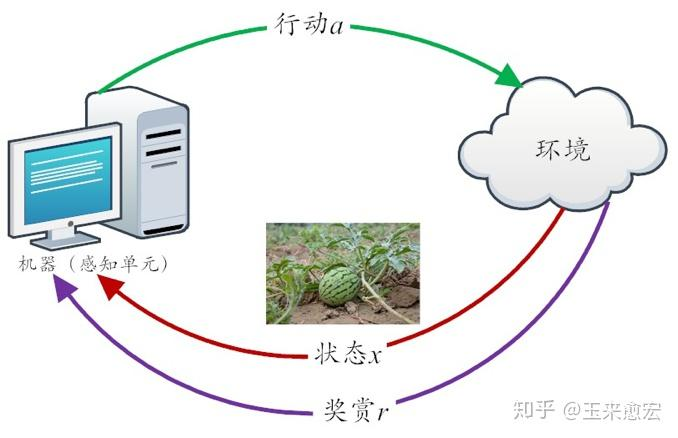
\includegraphics[width=1\textwidth]{figs/强化学习示意图.jpg}
\caption{强化学习示意图}
\label{强化学习示意图}
\end{figure}


在机器学习问题中，环境通常被规范为一个马可夫决策过程（Markov Decision Processes，MDP），许多强化学习算法就是在这种情况下使用动态规划技巧。

强化学习输出的就是一个由状态、奖励和行动组成的序列。而智能体的目标，就是让预期累积回报最大化。

3.7 强化学习强在哪里？
强化学习并不需要出现正确的“输入/输出对”，也不需要精确校正次优化的行为。深度学习“妙”在不需要做特征工程，而强化学习则“强”在不需要准备大量的训练样本，它重视的是环境给予的反馈。

强化学习更好地体现了人们（高智能动物）的为人处世原则：

“这世间，没有对错（非黑即白）之分，只有利害之度量”。
强化学习更专注于在线规划，需要在“探索”（在未知的领域）和“利用”（现有知识）之间找到平衡（Tradeoff）。强化学习中的“探索（exploration）-利用（exploitation）”的交换，这在多臂老虎机问题和有限MDP中研究得较多。

与强化学习相关的一则报道是，2017年10月，Google深度思维团队在著名学术期刊Nature（自然）上发表了一篇论文“Mastering the game of Go
without human knowledge（无须人类知识，精通围棋博弈）[4]，他们设计了AlphaGo（阿法狗）的升级版AlphaGo Zero（阿法元），阿法元从零（Tabula rasa[1]）开始，不需要人类任何历史围棋棋谱做指导，完全靠强化学习来参悟，自学成才，并以100∶0击败了阿法狗。

论文的第一作者、AlphaGo创始人之一大卫·席尔瓦（David Silver）指出，

阿法元远比阿法狗强大，因为它不再被人类的知识所局限，而是能够发现新知识，发现新策略。
这确实是机器学习进步的一个重要标志。更多有关强化学习的资料，请读者参阅参考资料[3]。

在强化学习的应用中，智能体通过与环境不断交互来获得奖励或惩罚，进而优化其决策过程。强化学习的应用领域非常广泛，包括但不限于以下几个方面：
\begin{itemize}
\item 在游戏对弈中，强化学习被用来训练智能体与自己或其他智能体对弈，从中学习最优策略。经典的例子包括AlphaGo，它通过与自我对弈不断优化决策策略，最终战胜了人类世界冠军。
\item 在自动驾驶中，智能体通过与环境（如道路、交通信号、行人等）互动，学习如何做出正确的驾驶决策，从而实现安全、有效的自动驾驶。
\item 在机器人控制领域，强化学习帮助机器人在复杂的环境中完成各种任务，如物体抓取、路径规划等。
\item 在智能推荐系统中，强化学习可以根据用户的历史行为和实时反馈，优化推荐策略，提供个性化的内容推荐。
\end{itemize}

总的来说，强化学习为解决复杂的动态决策问题提供了一种强大的工具，通过模拟试探和优化，智能体能够在未知和变化的环境中逐渐学习到最佳行为策略。


\newpage